%%=============================================================================
%% Onderzoek
%%=============================================================================

\chapter{Testen}
\label{ch:testen}

In dit hoofdstuk zullen de uitgevoerde experimenten en testen uiteengezet en besproken worden, volgens de richtlijnen aangehaald in Hoofdstuk~\ref{ch:methodologie}. Ze zullen gesorteerd staan volgens opstelling en gerangschikt in dezelfde volgorde als in Hoofdstuk~\ref{ch:opstellingen}.

\section{RFID}
Voor elk van volgende testen bestaat data over zowel de RSSI als het relatieve faseverschil. Het relatieve faseverschil heeft hetzelfde verloop als de RSSI, aangezien beide afhankelijk zijn van de afstand tussen de antenne en de tag, maar deze is meestal properder. In de uiteenzetting van de testen zal enkel 1 van deze 2 getoond worden, tenzij er een meerwaarde is van beide te tonen, maar de lezer moet er zich van bewust zijn dat beide voorhanden zijn en dat RSSI en fase wel eens door elkaar kan gebruikt worden. Ook is er bij alle statische testen data over in en uit de locatie, waarvan ook slechts 1 zal getoond worden tenzij beide een meerwaarde bied.

\subsection{1 antenne aan deurlijst}
%TODO

\subsection{2 antennes aan deurlijst}
\subsubsection{Deelhypothese}
Deze opstelling kan het voorbijkomen en de richting van een getagd asset waarnemen, genomen dat de afstand tussen de tag en de antenne voldoende klein is.

\subsubsection{Test 1: Oriëntatie van de tag}
In deze eerste test wordt de invloed van de oriëntatie van de tag tegenover de antennes bepaald, aangezien deze oriëntatie in theorie een invloed heeft op de gemeten RSSI waarde. De opstelling voor deze test is als volgt: 2 antennes zijn in een deuropening geplaatst, naast elkaar. Bij het binnenkomen wordt eerst antenne 1, en daarna antenne 2 gepasseerd. Er worden 4 oriëntaties onderzocht, nl. horizontaal (a) en verticaal (b) in hetzelfde vlak als de antennes, en horizontaal (c) en verticaal (d) loodrecht op het vlak van de antennes. Voor elk van deze deeltesten geld een afstand tussen de tag en de antenne van ~30cm. Bij elk scenario is zowel de richting in als uit getest, echter zullen deze resultaten enkel beide worden getoond als er een meerwaarde is.
In theorie zouden a en b ruwweg dezelfde resultaten moeten geven, terwijl c en d een lagere RSSI zouden moeten geven. Echter zou het in elk geval detecteerbaar moeten zijn.

\paragraph{a) Horizontaal in antennevlak}
\begin{minipage}{0.55\textwidth}
Uit bijhorende grafiek, die de tag toont die uit de locatie ging, is duidelijk een opeenvolging van pieken te zien. Dit met volgorde 2 (groen) -> 1 (blauw), wat inderdaad uit de locatie gaan is. Deze detectie is dus geslaagd. De piekhoogte is niet gelijk, ondanks dat de antennes hetzelfde type zijn. Dit is kalibreerbaar maar zoals zichtbaar is dit niet nodig voor een toepassing als deze.
\end{minipage}
\hfill
\begin{minipage}{0.42\textwidth}
	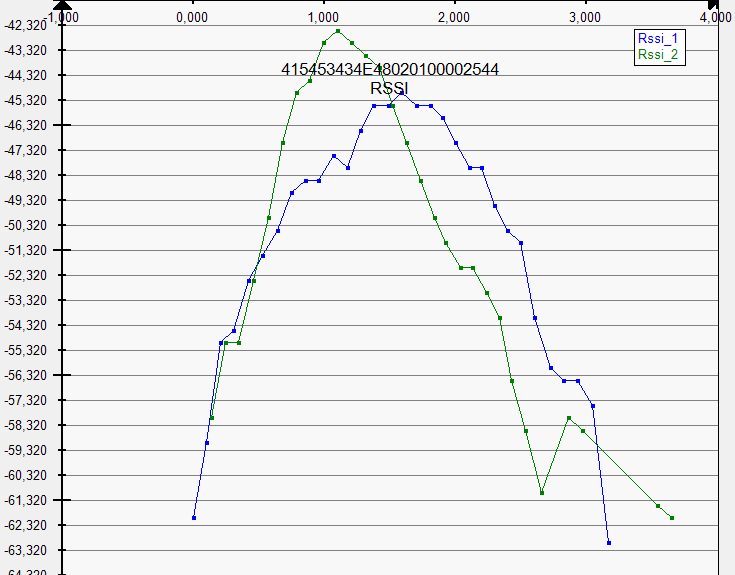
\includegraphics[width=\linewidth]{1a_uit_RSSI}
\end{minipage}

\paragraph{b) Verticaal in antennevlak}
\begin{minipage}{0.55\textwidth}
In deze grafiek is vrij gelijkaardig aan de vorige, wat theoretisch ook zou moeten. Er zijn duidelijk 2 pieken zichtbaar, in de juiste volgorde volgend de tag die uit de locatie gaat. Ook is de RSSI gelijkaardig (rond de -40 à -45 dBm).
\end{minipage}
\hfill
\begin{minipage}{0.42\textwidth}
	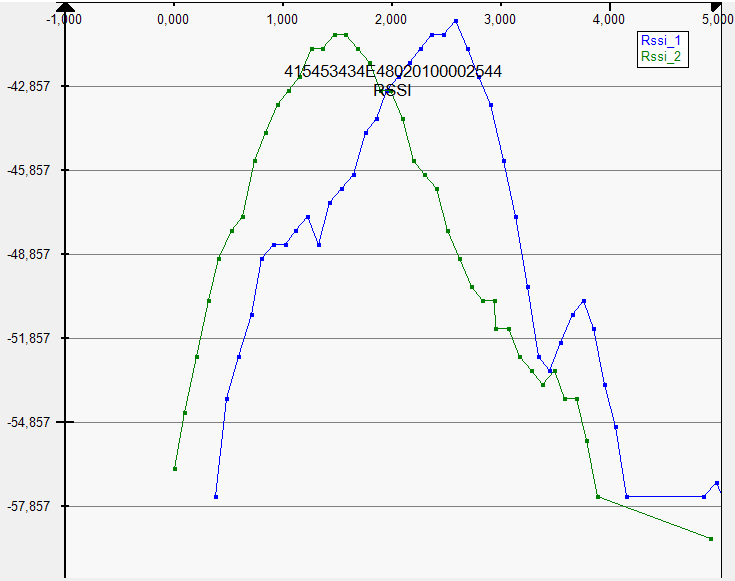
\includegraphics[width=\linewidth]{1b_uit_RSSI}
\end{minipage}

\paragraph{c) Horizontaal loodrecht op antennevlak}
\begin{minipage}{0.55\textwidth}
In deze grafiek is een beweging van de tag naar in de locatie weergegeven, hoewel de toppen duidelijk zichtbaar zijn, en in de correcte richting staan, is de top minder duidelijk afgelijnd en meer uitgerokken. Ditzelfde fenomeen is ook zichtbaar in de uit-richting. Ook liggen de toppen iets lager dan de toppen in de vorige 2 deeltests.
\end{minipage}
\hfill
\begin{minipage}{0.42\textwidth}
	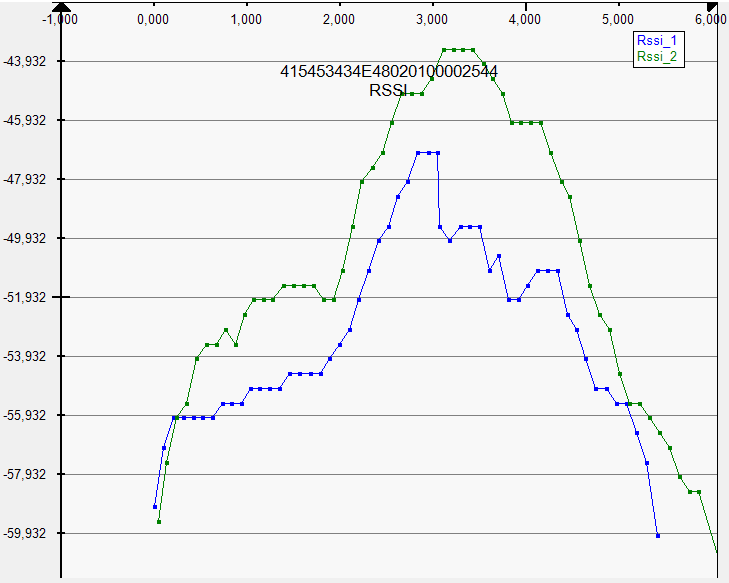
\includegraphics[width=\linewidth]{1c_in_RSSI}
\end{minipage}

\paragraph{d) Verticaal loodrecht op antennevlak}
\begin{minipage}{0.55\textwidth}
In deze grafiek in ook een beweging van de tag naar in de locatie weergegeven, en is het fenomeen van meer uitgerokken toppen nog beter zichtbaar. De uit richting vertoont wederom hetzelfde patroon. Deze deeltest ligt dus in lijn met de vorige, maar nog opvallender.
\end{minipage}
\hfill
\begin{minipage}{0.42\textwidth}
	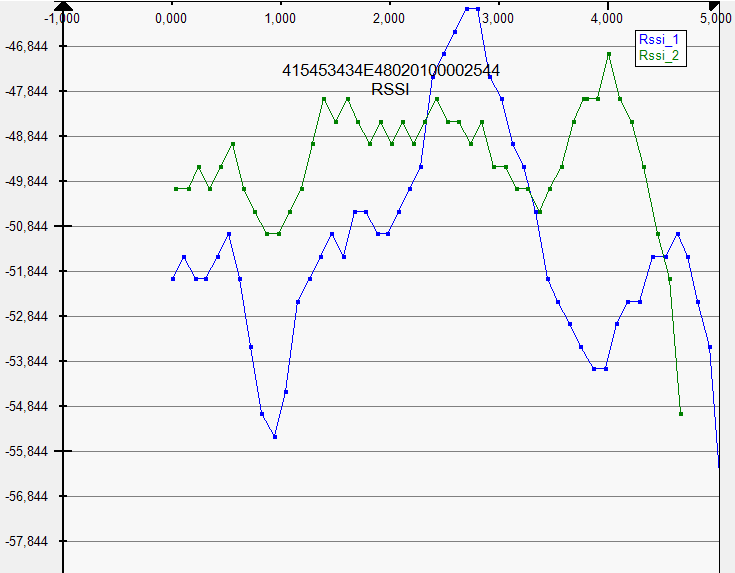
\includegraphics[width=\linewidth]{1d_in_RSSI}
\end{minipage}

\paragraph{Testconclusie}
Zoals verwacht is de detectie van de tag en de richting ervan goed zichtbaar en in elk geval correct gemeten. Ook is de meetkwaliteit minder als de tags niet in het vlak van de antenne liggen, daarom lijkt het aanbevolen dit zo veel mogelijk te vermijden.

\subsubsection{Test 2: Afstand tussen tag en antennes}
In deze test wordt de invloed van de afstand tussen de tag en de antennes gemeten, in theorie zou de RSSI van de piek lager moeten zijn als de tag verder van de antenne voorbij komt, en door de conische vorm van het meetveld van de vlakke antenne zouden de pieken meer moeten overlappen. De testopstelling is idem aan Test 1, de oriëntatie van de tag is constant gehouden op horizontaal in hetzelfde vlak als de antennes, en de richting is uit de locatie. De gemeten afstanden zijn 5cm afstand (zeer dicht) en 100cm afstand (zeer ver). Dit kan vergeleken worden met de resultaten van Test 1a, aangezien dit dezelfde opstelling betreft, op 30 cm afstand.

\paragraph{a) 5cm}
\begin{minipage}{0.55\textwidth}
Op deze grafiek is het verwachte resultaat te zien, 2 duidelijke pieken die licht verder uit elkaar liggen, en een hogere RSSI waarde hebben.
\end{minipage}
\hfill
\begin{minipage}{0.42\textwidth}
	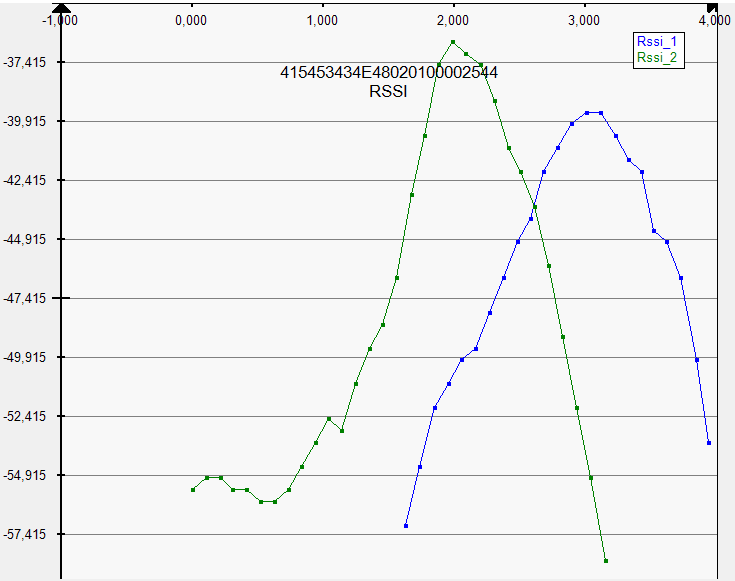
\includegraphics[width=\linewidth]{2a_RSSI}
\end{minipage}

\paragraph{b) 100cm}
\begin{minipage}{0.55\textwidth}
Deze grafiek is interessanter dan de vorige, het vermoeden dat de piek minder duidelijk ging zijn en ging overlappen is bevestigd. Uit deze meting kan niet meer afgeleid worden in welke richting de tag voorbij de antennes komt. Ook ligt de RSSI waarde beduidend lager.
\end{minipage}
\hfill
\begin{minipage}{0.42\textwidth}
	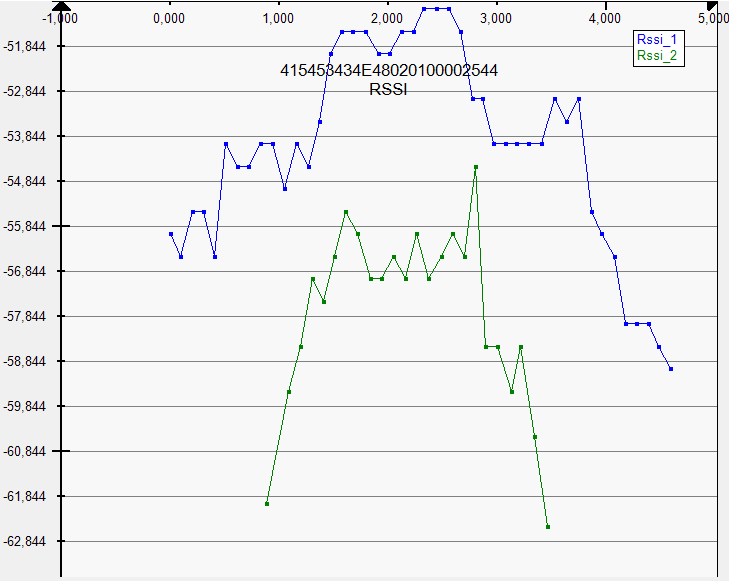
\includegraphics[width=\linewidth]{2b_RSSI}
\end{minipage}

\paragraph{Testconclusie}
Zoals werd vermoed is er een bepaalde restrictie op de afstand waarmee de tag de antennes kan voorbijkomen om een goede richtingsdetectie te hebben. 

\subsubsection{Test 3: Afstand tussen de 2 antennes}
Aangezien de reden van de overlappende pieken in vorige test het feit is dat het conische bereik van de 2 antennes elkaar te veel overlapt, is het logisch dat dit effect zal verminderen als deze 2 antennes verder van elkaar geplaatst worden, dit zal getest worden in deze 3e test. De opstelling is identiek aan de test 2, het enige verschil is dat de 2 antennes 20cm uit elkaar gezet zijn.

\paragraph{a) 5cm}
\begin{minipage}{0.55\textwidth}
Dit testresultaat toont wederom 2 mooie pieken, deze keer iets verder uit elkaar liggend door de afstand tussen de antennes, en dit met een lage RSSI waarde.
\end{minipage}
\hfill
\begin{minipage}{0.42\textwidth}
	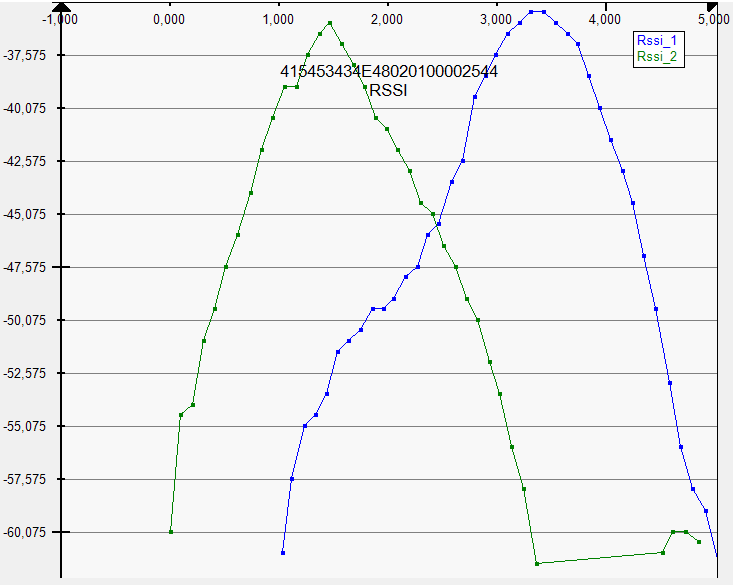
\includegraphics[width=\linewidth]{3a_RSSI}
\end{minipage}

\paragraph{b) 30cm}
\begin{minipage}{0.55\textwidth}
Hier zien we ongeveer hetzelfde als op de vorige grafiek, enkel licht meer uitgerokken en met een lagere RSSI waarde.
\end{minipage}
\hfill
\begin{minipage}{0.42\textwidth}
	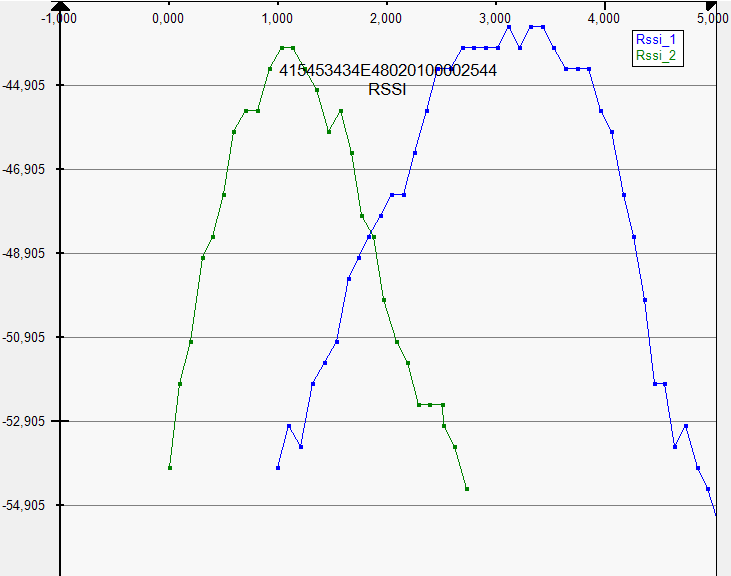
\includegraphics[width=\linewidth]{3b_RSSI}
\end{minipage}

\paragraph{b) 100cm}
\begin{minipage}{0.55\textwidth}
Dit resultaat is het voornaamste van deze test, we zien, zoals bij test 2, dat de pieken weer hard zijn uitgerokken, maar door de extra afstand tussen de antennes is de volgorde wel weer zichtbaar.
\end{minipage}
\hfill
\begin{minipage}{0.42\textwidth}
	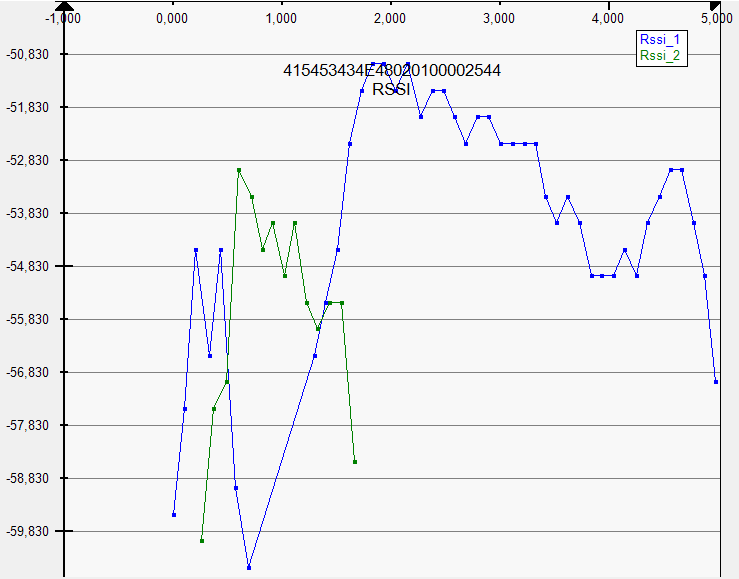
\includegraphics[width=\linewidth]{3c_RSSI}
\end{minipage}

\paragraph{Testconclusie}
Het blijkt inderdaad correct dat het verder uit elkaar plaatsen van de antennes een positief effect heeft op het uit elkaar trekken van de pieken in de RSSI curve, wat nodig is naarmate de tag verder van de antenne voorbij komt.

\subsubsection{Deelconclusie}
Deze opstelling slaagt er inderdaad in om een voorbijkomende tag en zijn richting te registreren, mits de afstand beperkt is, de hypothese is dus correct. Er kan echter wel aan toegevoegd worden dat, als de afstand niet meer voldoende klein is, dat de afstand tussen de antennes kan vergroot worden. Dit is in een reële situatie echter niet praktisch aangezien een deur meestal een beperkte breedte heeft. Voor een standaard deur zal dit geen probleem zijn aangezien de maximale afstand in een deur ook beperkt is, maar voor bv. een poortdoorgang kan dit wel problemen opleveren. In een gang met een quasi onbeperkte beschikbare breedte is dit wel mogelijk.

\subsection{1 antenne tegenover deur}
\subsubsection{Deelhypothese}
Deze opstelling kan het voorbijkomen en de richting van een getagd asset waarnemen, genomen dat de afstand tussen de antenne en de deur voldoende klein is zodat de antenne de tag kan registreren.

\subsubsection{Test 1: PoC}
Deze eerste test bestaat uit een proof of concept, hierin wordt getest of het op zijn minst mogelijk is om de richting van de bewegende tag te bepalen uit de gemeten data. 
In deze test wordt een antenne geplaatst tegen een muur, met daarvoor een kar met een tag op (horizontaal in het vlak van de antenne). Deze kar zal voor deze test achteruit en vooruit gerold worden. 

\paragraph{Resultaat}
Onderstaande grafieken tonen de verandering in RSSI van beide testen, met het rollen van de kar weg van de antenne links, en naar de antenne toe rechts. In deze grafieken is deze richting zeer mooi zichtbaar, de RSSI verlaagt als de kar wegrolt, en verhoogt als deze naar de antenne toe rolt.

\begin{minipage}{0.42\textwidth}
	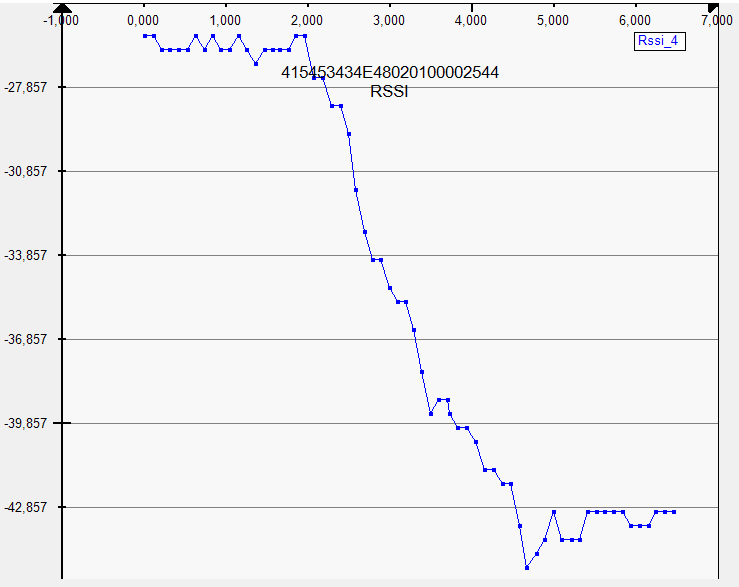
\includegraphics[width=\linewidth]{4c_RSSI}
\end{minipage}
\hfill
\begin{minipage}{0.42\textwidth}
	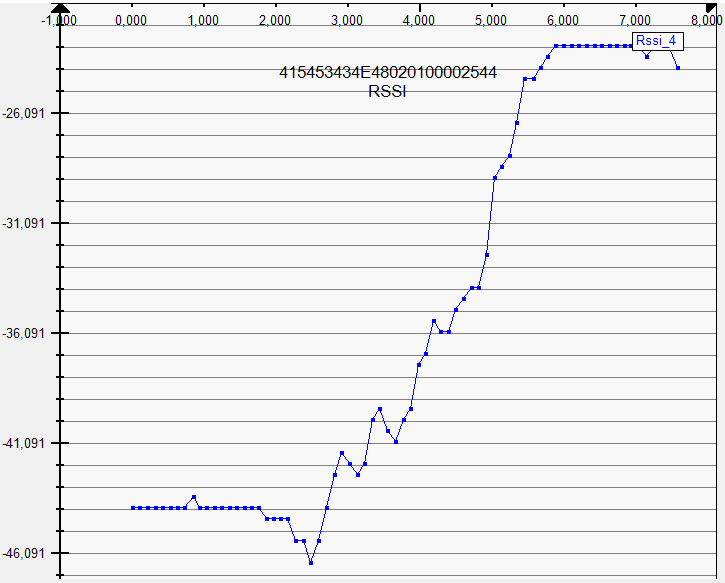
\includegraphics[width=\linewidth]{4d_RSSI}
\end{minipage}

\paragraph{Testconclusie}
Uit deze resultaten is zeer mooi te zien dat de richting van de verplaatsing op de lijn voor een antenne duidelijk zichtbaar is.

\subsubsection{Test 2: Variabele afstand tot deur}
In deze test wordt de opstelling realistischer gemaakt, de antenne wordt op respectievelijk 100 en 200 cm afstand van de deur geplaatst, en er wordt met de kar met bevestigde RFID tag van test 1 door de deur gereden, zowel in als uit de kamer, direct de hoek om. 

\paragraph{a) 100cm}
Hieronder is het binnenkomen (links) en het verlaten (rechts) van de locatie te zien, zoals duidelijk te zien is is de grafiek zeer veel minder duidelijk dan in de ideale situatie van test 1. Vermoedelijk is de 'staart' die niet in de meting past (rechts aanhangsel bij inwaarts en links bij uitwaarts) het gevolg van het feit dat de kar op dat moment 90° gedraaid in de kamer aanwezig is, resp. na en voor de draaibeweging door de deur. Op dit moment bevind de tag zich in het leesveld van de antenne, maar niet meer in hetzelfde vlak. Deze onderlinge oriëntatie zorgt voor een slechte RSSI waarde, zoals aangetoond tijdens test 1 van de vorige opstelling. Voor de duidelijkheid van de 'uit' meting is dit niet zo zeer een probleem, maar wel voor de 'in' meting.

\begin{minipage}{0.42\textwidth}
	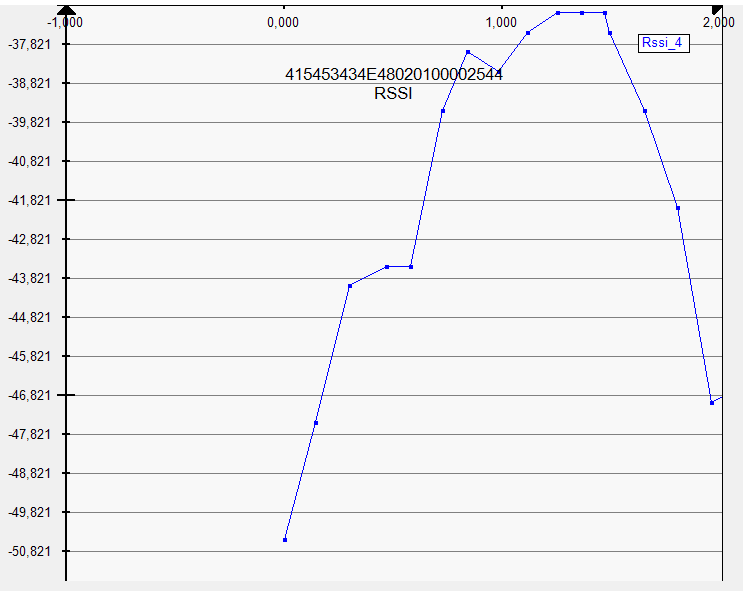
\includegraphics[width=\linewidth]{5a_in_RSSI}
\end{minipage}
\hfill
\begin{minipage}{0.42\textwidth}
	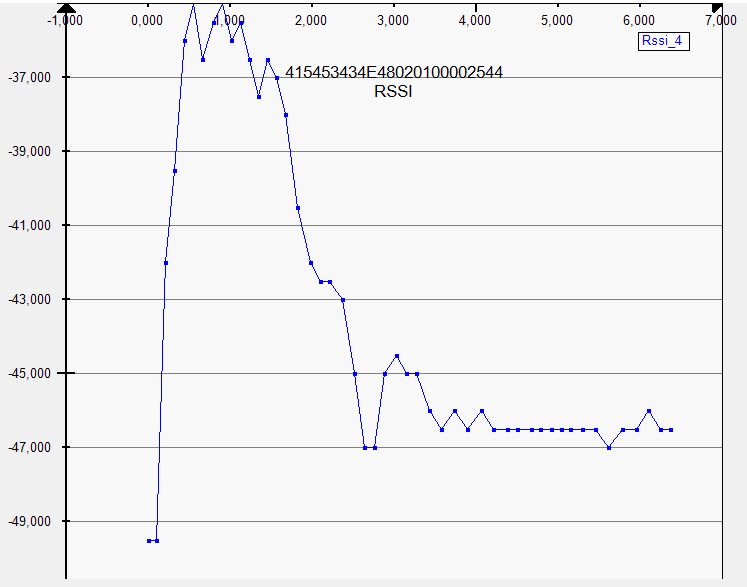
\includegraphics[width=\linewidth]{5a_uit_RSSI}
\end{minipage}

\paragraph{b) 200cm}
Hieronder is wederom het binnenkomen (links) en het verlaten (rechts) van de locatie te zien. In dit geval is de onduidelijkheid zichtbaar in vorige deeltest nog extremer zichtbaar. Alhoewel het in theorie de richting nog steeds eenduidig zichtbaar is, is het nog minder duidelijk, en deze onduidelijkheid vergroot naarmate de tussenliggende afstand groter wordt. Ook de RSSI waarde ligt logischerwijs lager.

\begin{minipage}{0.42\textwidth}
	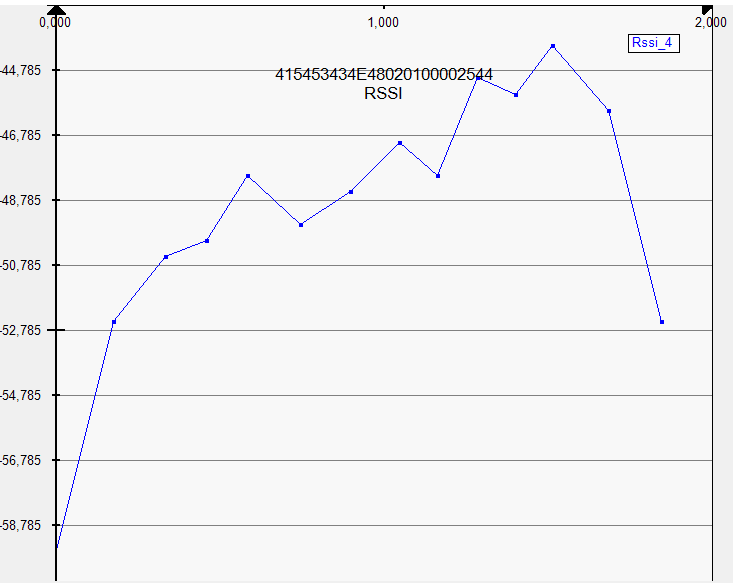
\includegraphics[width=\linewidth]{5b_in_RSSI}
\end{minipage}
\hfill
\begin{minipage}{0.42\textwidth}
	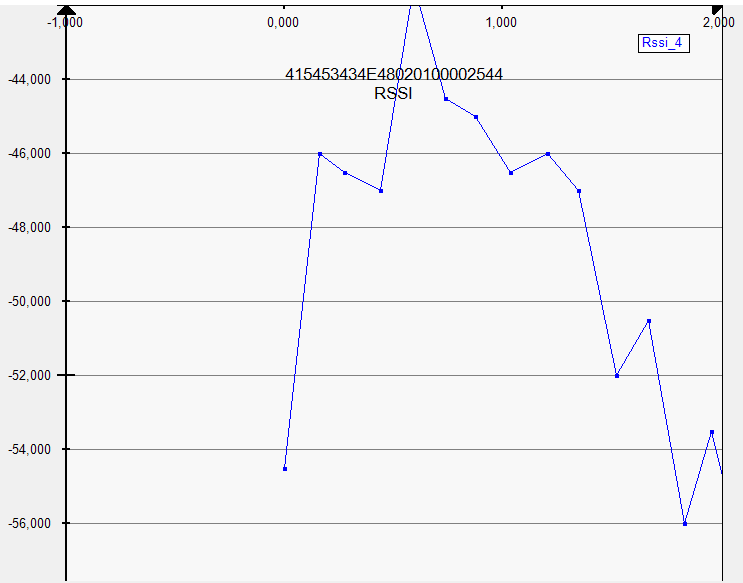
\includegraphics[width=\linewidth]{5b_uit_RSSI}
\end{minipage}

\paragraph{Testconclusie}
Deze testen tonen aan dat de meting in een realistisch scenario veel minder optimaal is als in het optimaal scenario van test 1 aangezien de meetpunten rond het dichter/verder komen voor onduidelijkheden zorgen die niet eenduidig uit de data te halen zijn.

\subsubsection{Test 3: Langere meetafstand}
Aangezien een simpele draai rond het deurgat te slechte data oplevert om eenduidig de richting te bepalen, kan het een idee zijn om de kar langer op de lijn van de antenne te laten rijden om zo het relatieve aantal van meetpunten voor de richtingsdetectie op te krikken tegenover de meetpunten bij het in- en uit stappen van het meetbereik van de antenne. Dit wordt in volgende test bekeken, hierbij is de opstelling idem aan test 2b, maar zal de kar tot tegen de antenne rijden alvorens af te slaan.

\paragraph{Resultaat}
Onderstaande grafieken tonen wederom de verandering in RSSI van beide richtingen, met het rollen van de kar naar de antenne links, en weg van de antenne rechts. Alhoewel de 'staarten' uit test 2 nog steeds zichtbaar zijn, overheersen ze de grafiek niet meer en dus is deze grafiek veel eenduidiger en kan uit de richting van de scheefheid de richting van verplaatsing worden afgeleid.

\begin{minipage}{0.42\textwidth}
	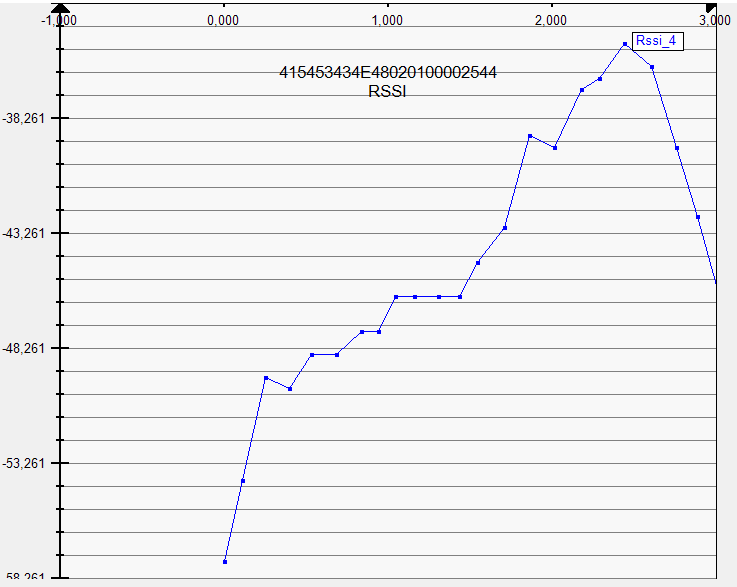
\includegraphics[width=\linewidth]{5c_in_RSSI}
\end{minipage}
\hfill
\begin{minipage}{0.42\textwidth}
	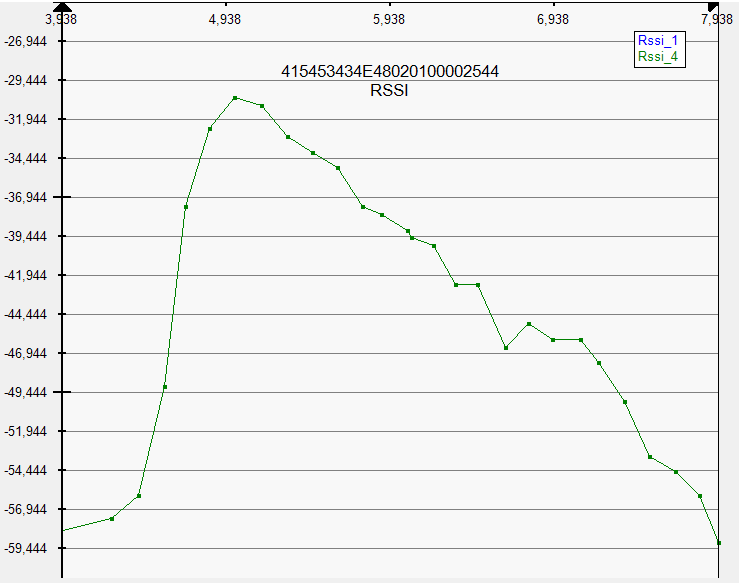
\includegraphics[width=\linewidth]{5c_uit_RSSI}
\end{minipage}

\paragraph{Testconclusie}
Het vermoeden dat de resultaten beter zijn als er verder op de lijn voor de antenne wordt gewandeld lijkt te zijn bevestigd met deze test.

\subsubsection{Deelconclusie}
In ideale omstandigheden blijkt dit concept zeer goed te werken, echter zijn er enkele neveneffecten van een realistische draai door een deur die moeten gecompenseerd worden met een langere lengte op de lijn voor de antenne te lopen. De vooropgestelde hypothese is dus niet correct en moet aangevuld worden met deze nieuwe informatie. In praktijk wilt dit zeggen dat dit niet werkt voor een normale deuropening en vorige opstelling dus gebruikt zal moeten worden. Echter kan het wel een oplossing zijn voor een (korte) gang of dergelijke waar de assets sowieso door moeten om een berging of magazijn te bereiken, want vanaf er enige afstand wordt gedaan werkt dit wel zeer goed. 

\subsection{1 tag aan deurlijst}
%TODO


\section{BLE}

\subsection{1 gateway per locatie}
%TODO

\subsection{Meerdere gateways per locatie}
%TODO

\subsection{Gateways in rasteropstelling}
%TODO

\subsection{1 beacon per locatie, midden van locatie}
%TODO

\subsection{1 beacon per locatie, aan deur}
%TODO

\subsection{Meerdere locatiebeacons per locatie}
%TODO

\subsection{Beacons in rasteropstelling}
%TODO

\subsection{Beacons op intervallen in de gang}
%TODO
